\documentclass[a4paper]{article}
\usepackage{a4wide,amssymb,epsfig,latexsym,multicol,array,hhline,fancyhdr}
\usepackage{vntex}
\usepackage{amsmath}
\usepackage{lastpage}
\usepackage[lined,boxed,commentsnumbered]{algorithm2e}
\usepackage{enumerate}
\usepackage{color}
\usepackage{graphicx}							% Standard graphics package
\usepackage{array}
\usepackage{tabularx, caption}
\usepackage{multirow}
\usepackage{multicol}
\usepackage{rotating}
\usepackage{graphics}
\usepackage{geometry}
\usepackage{setspace}
\usepackage{epsfig}
\usepackage{tikz}
\usepackage{tkz-graph}
\usetikzlibrary{arrows.meta}
\usepackage{enumitem}
\usepackage{algorithmic}
\usepackage{xcolor}
\usepackage{algorithm}
\usetikzlibrary{arrows,snakes,backgrounds}
\usepackage{hyperref}
\hypersetup{urlcolor=blue,linkcolor=black,citecolor=black,colorlinks=true} 
%\usepackage{pstcol} 								% PSTricks with the standard color package
\usepackage{listings}

\newtheorem{theorem}{{\bf Theorem}}
\newtheorem{property}{{\bf Property}}
\newtheorem{proposition}{{\bf Proposition}}
\newtheorem{corollary}[proposition]{{\bf Corollary}}
\newtheorem{lemma}[proposition]{{\bf Lemma}}

\AtBeginDocument{\renewcommand*\contentsname{Contents}}
\AtBeginDocument{\renewcommand*\refname{References}}
%\usepackage{fancyhdr}
\setlength{\headheight}{40pt}
\pagestyle{fancy}
\fancyhead{} % clear all header fields
\fancyhead[L]{
 \begin{tabular}{rl}
    \begin{picture}(25,15)(0,0)
    \put(0,-8){
\includegraphics[width=8mm, height=8mm]{hcmut.png}}
    %\put(0,-8){\epsfig{width=10mm,figure=hcmut.eps}}
   \end{picture}&
	%
\includegraphics[width=8mm, height=8mm]{hcmut.png} & %
	\begin{tabular}{l}
		\textbf{\bf \ttfamily University of Technology, Ho Chi Minh City}\\
		\textbf{\bf \ttfamily Faculty of Computer Science and Engineering}
	\end{tabular} 	
 \end{tabular}
}
\fancyhead[R]{
	\begin{tabular}{l}
		\tiny \bf \\
		\tiny \bf 
	\end{tabular}  }
\fancyfoot{} % clear all footer fields
\fancyfoot[L]{\scriptsize \ttfamily Assignment for Discrete Structures for Computing - Academic year 2023 - 2024}
\fancyfoot[R]{\scriptsize \ttfamily Page {\thepage}/\pageref{LastPage}}
\renewcommand{\headrulewidth}{0.3pt}
\renewcommand{\footrulewidth}{0.3pt}


%%%
\setcounter{secnumdepth}{4}
\setcounter{tocdepth}{3}
\makeatletter
\newcounter {subsubsubsection}[subsubsection]
\renewcommand\thesubsubsubsection{\thesubsubsection .\@alph\c@subsubsubsection}
\newcommand\subsubsubsection{\@startsection{subsubsubsection}{4}{\z@}%
                                     {-3.25ex\@plus -1ex \@minus -.2ex}%
                                     {1.5ex \@plus .2ex}%
                                     {\normalfont\normalsize\bfseries}}
\newcommand*\l@subsubsubsection{\@dottedtocline{3}{10.0em}{4.1em}}
\newcommand*{\subsubsubsectionmark}[1]{}
\makeatother

% Define a custom color
\definecolor{codegreen}{rgb}{0,0.6,0}
\definecolor{codegray}{rgb}{0.5,0.5,0.5}
\definecolor{codepurple}{rgb}{0.58,0,0.82}
\definecolor{backcolour}{rgb}{0.95,0.95,0.92}

% Define a custom style
\lstdefinestyle{myStyle}{
    backgroundcolor=\color{backcolour},   
    commentstyle=\color{codegreen},
    keywordstyle=\color{magenta},
    numberstyle=\tiny\color{codegray},
    stringstyle=\color{codepurple},
    basicstyle=\ttfamily\footnotesize,
    breakatwhitespace=false,         
    breaklines=true,                 
    keepspaces=true,                 
    numbers=left,       
    numbersep=5pt,                  
    showspaces=false,                
    showstringspaces=false,
    showtabs=false,                  
    tabsize=2,
}
% Use \lstset to make myStyle the global default
\lstset{style=myStyle}

\begin{document}

\begin{titlepage}
\begin{center}
VIETNAM NATIONAL UNIVERSITY, HO CHI MINH CITY \\
UNIVERSITY OF TECHNOLOGY \\
FACULTY OF COMPUTER SCIENCE AND ENGINEERING
\end{center}

\vspace{1cm}

\begin{figure}[h!]
\begin{center}

\includegraphics[width=3cm]{hcmut.png}
\end{center}
\end{figure}

\vspace{1cm}


\begin{center}
\begin{tabular}{c}
\multicolumn{1}{c}{\textbf{{\Large MATHEMATICAL MODELING(CO2011)}}}\\

~~\\
\hline
\\
\multicolumn{1}{l}{\textbf{{\Large Assignment}}}\\
\\
\textbf{{\Huge Stochastic Programming and }}\\
\textbf{{\Huge Applications}}
\\
\textbf{{\Huge }}\\
\\
\hline
\end{tabular}
\end{center}

\vspace{3cm}

\begin{table}[h]
\begin{tabular}{rrl}
\hspace{5 cm} & Advisor: & PhD. Nguyễn Tiến Thịnh.\\
& Students: & Nguyễn Gia Nguyên - 2212303.\\
& & Nguyễn Trung Phú - 2212592.\\
 & &Nguyễn Lê Đức Hiếu - 2210997.\\
 &&Lê Trường Thịnh - 2213282.\\
 &&Nguyễn Kim Đại Nghĩa - 2212229.\\
 &&Nguyễn Thành Nhân - 2012522.\\

\end{tabular}
\end{table}

\begin{center}
{\footnotesize HO CHI MINH CITY, DECEMBER 2023}
\end{center}
\end{titlepage}


%\thispagestyle{empty}

\newpage
\tableofcontents
\newpage


%%%%%%%%%%%%%%%%%%%%%%%%%%%%%%%%%
\section{Member list \& Workload}

\begin{center}
\begin{tabular}{|c|c|c|l|c|}
\hline
\textbf{No.} & \textbf{Fullname} & \textbf{Student ID} & \textbf{Problems} & \textbf{Percentage of work}\\
\hline 
%%%%%Student 1%%%%%%%%%%
\multirow{3}{*}{1} & \multirow{3}{*}{Nguyễn Lê Đức Hiếu} & \multirow{3}{*}{2210997} & - Giải quyết problem 1,& \multirow{3}{*}{100\%}\\
& &  & bao gồm:&\\
 & &  & + Tổng hợp lý thuyết &\\
 & &  & + Xử lý giai đoạn 1 &\\
\hline 
%%%%%Student 2%%%%%%%%%%%
\multirow{3}{*}{2} & \multirow{3}{*}{Nguyễn Kim Đại Nghĩa} & \multirow{3}{*}{2212229} & - Giải quyết problem 1,& \multirow{3}{*}{100\%}\\
& &  & bao gồm:&\\
 & &  & + Xử lý giai đoạn 2 &\\
 & &  & + Tổng hợp và chỉnh sửa&\\
 & &  & thuật toán &\\
\hline
%%%%%Student 3%%%%%%%%%%%
\multirow{3}{*}{3} & \multirow{3}{*}{Nguyễn Gia Nguyên} & \multirow{3}{*}{2212303} & -  Soạn bài cáo bài tập lớn & \multirow{3}{*}{100\%}\\
 & &  & - Phân chia, và hỗ trợ các&\\
 & &  &thành viên hoàn thành công&\\
  & & &việc của mình &\\
\hline 
%%%%%Student 4%%%%%%%%%%%
\multirow{3}{*}{4} & \multirow{3}{*}{Lê Trường Thịnh} & \multirow{3}{*}{2213282} & - Giải quyết problem 2,& \multirow{3}{*}{100\%}\\
& &  &bao gồm:&\\
 & &  & + Soạn code giải thuật&\\
  & &  &"Cycle canceling"&\\
 & &  & + Tổng hợp lý thuyết&\\
\hline
%%%%%Student 5%%%%%%%%%%%
\multirow{3}{*}{5} & \multirow{3}{*}{Nguyễn Trung Phú} & \multirow{3}{*}{2212592} & - Giải quyết problem 2,& \multirow{3}{*}{100\%}\\
& &  &bao gồm:&\\
 & &  & + Soạn code giải thuật&\\
 & &  &"Successive Shortest Path"&\\
 & &  & - Tổng hợp lý thuyết&\\
\hline
%%%%%Student 6%%%%%%%%%%%
\multirow{3}{*}{6} & \multirow{3}{*}{Nguyễn Thành Nhân} & \multirow{3}{*}{2012522} & - Giải quyết problem 2:& \multirow{3}{*}{100\%}\\
 & &  & Thực hiện so sánh hiệu năng&\\
 & &  & của giải thuật "Successive &\\
 & &  & Shortest Path" với giải thuật&\\
 & &  &  "Cycle canceling"&\\
\hline
\end{tabular}
\end{center}
File log chi tiết về tiến trình làm việc, nội dung thảo luận - \textcolor{blue}{Weekly\_log.txt} đã được đính kèm cùng bài báo cáo này
%%%%%%%%%%%%%%%%%%%%%%%%%%%%%%%%%
\section{Stochastic Programming}
	\subsection{Cơ sở lý thuyết}
 \subsubsection{Khái niệm}
\begin{itemize}
    \item \textbf{Linear programming (LP)} (quy hoạch tuyến tính) là bài toán tối ưu hóa, trong đó hàm mục tiêu (objective function) và các điều kiện ràng buộc đều là tuyến tính.
\end{itemize}
\begin{itemize}
    \item \textbf{Stochastic Programming (SP) } (Quy hoạch ngẫu nhiên) là bài toán về việc ra quyết định trong điều kiện không chắc chắn. Xem nó dưới dạng 'Lập trình toán học (Tối ưu hóa) với các tham số ngẫu nhiên'.
\end{itemize}
\begin{itemize}
    \item \textbf{Stochastic linear programs} (quy hoạch tuyến tính ngẫu nhiên) là các chương  tuyến tính (tức là hàm mục tiêu của nó là tuyến tính) trong đó một số dữ liệu bài toán có thể được coi là bất định, không chắc chắn.
\end{itemize}
Dạng cơ bản quy hoạch tuyến tính ngẫu nhiên là:
\begin{equation}
    \textcolor{blue} {\text{Minimize Z} = g(x) = f(x) = c^T\cdot x \quad \text{s.t. } A \cdot x = b} \label{eq:einstein} \tag{\textcolor{blue}{1}}
\end{equation}


\quad {Với $\textcolor{blue}{x = (x_1, x_2, ..., x_n)}$ là các biến quyết định} .\\

\quad Với ma trận $\textcolor{blue}{A}$ và vector $\textcolor{blue}{b}$ làm ràng buộc của biến quyết.\\

\quad Các tham số ngẫu nhiên $\textcolor{blue}{T, h}$ trong $\textcolor{blue}{Tx \geq h}$ là xác xuất của biến quyết định.

\subsubsection{Bài toán Mô hình Tối ưu Hóa Tuyến Tính một giai đoạn }

\textbf SLP với một giai đoạn (1-SLP) được định nghĩa như sau:

Xem xét bài toán \textcolor{blue}{\(LP(\alpha)\)}, với tham số vector ngẫu nhiên  \textcolor{blue}{\(\alpha\)}:
\begin{equation}
    \textcolor{blue}{\text{Minimize Z} = g(x) = f(x) = c^T \cdot x = \sum_{j=1}^{n} c_j x_j} \label{eq:einstein} \tag{\textcolor{blue}{2}}
\end{equation}


s.t:

\[
\begin{aligned}
&\textcolor{blue}{Ax = b }\quad \text{(ràng buộc chắc chắn}) \\
&\textcolor{blue}{Tx \geq h} \quad \text{(ràng buộc ngẫu nhiên)}
\end{aligned}
\]

với giả sử rằng:

\begin{enumerate}
    \item Ma trận \textcolor{blue}{$(T = T(\alpha))$} và vector \(h = h(\alpha)\) biểu diễn sự bất định thông qua ràng buộc ngẫu nhiên:
    
   \[
\textcolor{blue}{T(\alpha) x \geq h(\alpha) \Leftrightarrow \alpha_1 x_1 + \ldots + \alpha_n x_n \geq h(\alpha)}
\]

    
    \item Giá trị của \textcolor{blue}{\((T, h)\)} chưa được biết; chúng là không xác định trước khi một trường hợp của mô hình xuất hiện. \textcolor{blue}{$(h=h(\alpha))$)} chỉ phụ thuộc vào ngẫu nhiên \textcolor{blue}{\(\alpha_j\)}.
    
    \item Sự bất định được biểu thị thông qua phân phối xác suất của các tham số ngẫu nhiên \textcolor{blue}{\((\alpha_j) = \alpha\)}.
\end{enumerate}

Chúng ta đối mặt với các vấn đề trong đó vector \(x = (x_1, x_2, \ldots, x_n) \in X\) của các biến quyết định phải được đưa ra trước khi biến thực của vector tham số \(\alpha \in \Omega\) được biết.\\

\quad Thông thường thì, chúng ta đặt các giới hạn dưới và giới hạn trên cho \(x\) thông qua miền \textcolor{blue}{\(X = \{x \in \mathbb{R}^n : l \leq x \leq u\}\)}.\\

Các Tiếp Cận Trong Lập Trình Tuyến Tính Ngẫu Nhiên

\begin{enumerate}
    \item \textbf{Ràng Buộc Xác Suất (Chance) LP:}
    \begin{itemize}
          \item Chúng ta có thể thay thế $T x \geq h$ bằng ràng buộc xác suất $P[T x \geq h] \geq p^2$ đáng tin cậy nhất định. 
          \item Rủi ro sau đó được xử lý một cách cẩn thận, và được định nghĩa là 
          \textcolor{blue}{$$r_x := P[\text{Not} (T x \geq h)] = P[T x \leq h] \leq 1 - p$$}\\
          \textcolor{blue}{$(1 - p)$} được coi rủi ro chập nhận tối đa.
    
    \end{itemize}
\item Trong trường hợp \textcolor{blue}{$T(\alpha) x \leq h(\alpha)$ }

\quad Cho mọi trường hợp \textcolor{blue}{$(T_s, h_s)$, $s = 1, \ldots, S$}, giải bài toán:
\textit{\textcolor{blue}{$$\text{Minimize f(x)} = c^T \cdot x \mid \text{với điều kiện } A x = b, T_s x \leq h_s$$ }} 
\begin{itemize}
\item \textbf{Ưu điểm:} Mỗi trường hợp là một LP. 
\item \textbf{Nhược điểm:} Phân phối rời rạc $\rightarrow$ mô hình LP số nguyên kết hợp. (có thể là mô hình không lồi).
\end{itemize}
\end{enumerate}
\subsubsection{Bài toán mô hình tối ưu hóa tuyến tính hai giai đoạn}
\begin{enumerate}
    \item Bài toán mô hình ngẫu nhiên hai giai đoạn\\
    \textbf Chương trình ngẫu nhiên hai giai đoạn (2-SP) được mở rộng từ (2) có dạng
 \textcolor{blue}{$$\text{2 - SP}: \min_x g(x) \text{ với } g(x) = f(x) + E^\omega[v(x, \omega)] $$}
trong đó \(\textcolor{blue}{ x = (x_1, x_2, \ldots, x_n)} \) là các biến quyết định giai đoạn đầu tiên,
\( \textcolor{blue}{f(x)} \) có thể tuyến tính hoặc không, là một phần của hàm mục tiêu tổng \(\textcolor{blue}{g(x)} \).
\begin{itemize}
    \item  \( \textcolor{blue}{Q(x) := E^\omega[v(x, \omega)]} \) của một hàm
    \( \textcolor{blue}{v : \mathbb{R}^n \times \mathbb{R}^S \rightarrow \mathbb{R} }\)
    do ảnh hưởng của các  \( \omega \),là giá trị tối ưu của một vấn đề giai đoạn thứ hai cụ thể:
    \[ \textcolor{blue}{\min_{y \in \mathbb{R}^p} qy \, | \, \text{subject to } T \cdot x + W \cdot y = h. } \]
    \item Vectơ \( \textcolor{blue}{\alpha = \alpha(\omega) }\) và \( \textcolor{blue}{y = y(\omega)} \) được gọi là biến bất , chỉ biết sau khi thực nghiệm \( e \).
\end{itemize}
Chúng ta tối thiểu hóa chi phí kỳ vọng tổng cộng \(\textcolor{blue}{ g(x) = f(x) + Q(x)} \) trong khi đảm bảo
\[\textcolor{blue}{ W \cdot y(\omega) = h(\omega) - T(\omega) \cdot x }\]
Ở đây, \( \textcolor{blue}{W} \) được gọi là ma trận phục hồi kích thước \( m \times p \), và chúng ta bắt đầu với trường hợp đơn giản của \( \textcolor{blue}{m = 1} \),
\( \textcolor{blue}{q }\) là vector chi phí phục hồi đơn vị, có cùng kích thước như \(\textcolor{blue}{ y }\), và \( \textcolor{blue}{y = y(\omega) \in \mathbb{R}^p} \).

\textbf{Cụ thể:}
\begin{itemize}
    \item Mục tiêu tổng lớn \(\textcolor{blue}{ g(x)} \) được tạo ra bởi \(\textcolor{blue}{ f(x)} \) và \(\textcolor{blue}{ Q(x)} \). Ở đây, \(\textcolor{blue}{ y }\) là vectơ quyết định của một vấn đề LP giai đoạn thứ hai, giá trị của \( \textcolor{blue} {y} \) phụ thuộc vào thực hiện của \( \textcolor{blue}{(T, h) := (T(\omega), h(\omega))} \). Biến quyết định phục hồi \( \textcolor{blue}{y(\omega)} \) ∼ các hành động sửa đổi, chẳng hạn như việc sử dụng các nguồn lực sản xuất thay thế (làm thêm giờ...).
    \item Đo lường rủi ro lượng: kích thước của độ chệch \(\textcolor{blue}{ h(\omega) - T(\omega) \cdot x }\) có liên quan.
    \item Ở đây, RỦI RO được mô tả bằng  recourse costs kỳ vọng \( Q(x) \) của biến quyết định \( x \).
\end{itemize}
    \item Bài toán mô hình tuyến tính ngẫu nhiên hai giai đoạn\\
   \textbf{ Mô hình Tối ưu Hóa Tuyến Tính Hai Giai Đoạn với Hậu Quả (2-SLPWR) - (dạng đơn giản):}


\[ \textcolor{blue}{
\min_{x\in X} c^T \cdot x + \min_{y(\omega)\in Y} E^\omega[q \cdot y]}
\]
hoặc:
\[\textcolor{blue}{
\min_{x\in X, y(\omega)\in Y} E^\omega[c^T \cdot x + v(x, \omega)]}
\]

s.t:
\begin{align*}
&\textcolor{blue}{A x = b} \quad \text{(Ràng buộc Giai Đoạn Thứ Nhất)} \\
&\textcolor{blue}{T(\omega) \cdot x + W \cdot y(\omega) = h(\omega)} \quad \text{ (Ràng buộc Giai Đoạn Thứ hai)} 
\end{align*}

\textcolor{blue}{$y = y(x, \omega) \in \mathbb{R}_+^p $}+\quad \text{là biến quyết định cho quyết định } $\textcolor{blue}{x} \text{ và sự hiện thực của } \textcolor{blue}{\omega}.$

\\

 \textbf{Mô hình Tối ưu Hóa Tuyến Tính Hai Giai Đoạn với Hậu Quả (dạng chuẩn):}

2-SLPWR dạng chuẩn:


\[\textcolor{blue}{
\min_{x} g(x)}\]
\[\textcolor{blue}{\text{khi} \quad g(x) = c^T \cdot x + v(y)}
\]
\begin{align*}
&\textcolor{blue}{st: Ax = b} \quad \text{khi} \quad \textcolor{blue}{x \in X \subseteq \mathbb{R}^n, x \geq 0} \\
&\textcolor{blue}{v(z) = \min_{y\in \mathbb{R}_+^p} qy} \quad \text{ s.t} \quad \textcolor{blue}{W \cdot y = h(\omega) - T(\omega) \cdot x = z}
\end{align*}

\textcolor{blue}{$y = y(x, \omega) \in \mathbb{R}_+^p $}+\quad \text{là biến quyết định cho quyết định } $\textcolor{blue}{x} \text{ và sự hiện thực của } \textcolor{blue}{\omega}.$\\
Mục Tiêu:\\
1. Tối thiểu hóa chi phí hậu quả kỳ vọng \(Q(x)\):\\

\textcolor{blue}{$
Q(x) = E^\omega[v(x, \omega)]$ }


2. Thiết kế biến quyết định thứ hai \textcolor{blue}{\((y\omega)\)}:
Duyệt, điều chỉnh, hoặc phản ứng với ràng buộc gốc một cách thông minh (biện pháp hậu quả).

3. Giải pháp tối ưu:
Giá trị tối ưu của LP giai đoạn thứ hai là \textcolor{blue}{\(v^* = v(y^*)\), với \(y^*\)} là giải pháp tối ưu.
Giá trị tối ưu toàn bộ là \textcolor{blue}{\(c^T \cdot x^* + v(y^*)\)}.
\end{enumerate}







\subsection{Giải quyết problem 1}

\subsubsection{Các khái niệm có trong yêu cầu}
%%%%%%%%%%%%%%%%%%%%%%%
    Mô hình lập trình tuyến tính ngẫu nhiên hai giai đoạn (2 - SLPWR) được áp dụng rộng rãi trong bối cảnh sản xuất: quyết định tới việc lập kế hoạch sản xuất và quản lý hàng tồn kho khi xét đến nhu cầu, chi phí không chắc chắn liên quan đến sản xuất, đặt hàng linh kiện và giá trị thu hồi.Ở bài toán này chúng ta sẽ giải quyết trong 2 giai đoạn:

    \begin{enumerate}
        \item Giai đoạn 1: đưa ra các quyết định "here and now", để từ đó có thể tăng độ hiệu quả và không bị phụ thuộc vào những thông tin không chắc chắn hay những yếu tố ngẫu nhiên ảnh hưởng đến tối ưu chi phí \\
    
%%%%%%%%%%%%%%%%%%%%%%%%%%%%%%%5

\begin{minipage}{0.8\textwidth}
    \setlength{\parindent}{20pt}   
    Gọi \textcolor{blue}{$x$} là số lượng hàng đặt trước đã tối ưu từ các nhà cung cấp trước đó:
   \textcolor{blue}{ \[ x = (x_1, x_2, \ldots, x_{i}) \text{ với } i = 1,2,3, \ldots, n \]}
 \end{minipage}   \\
\begin{minipage}{0.8\textwidth}  
    \setlength{\parindent}{20pt}   
    Gọi \textcolor{blue}{$b$} là chi phí giảm thiểu khi đặt hàng trước:
   \textcolor{blue}{ \[ b = (b_1, b_2, \ldots, b_{j}) \text{ với } j = 1,2,3, \ldots, m \]}
    
    \textcolor{blue}{$Q(x)$} là lợi nhuận dự kiến khi quyết định lập kế hoạch sản xuất:
    \textcolor{blue}{\[ Q(x) = E[Z(x,y)] = E_{\omega}[x, \omega] \]}
    
    Qua những tố trên, ta đặt ra bài toán giải quyết tối ưu chi phí:
    \textcolor{blue}{\[ \min g(x,y,z) = b^T \cdot x  + Q(x) = b^T \cdot x + E[Z(z)] \]}
    
    \begin{minipage}{\textwidth}
        \setlength{\parindent}{20pt}
        Trong đó: \textcolor{blue}{$Q(x) = E_{\omega}[Z] = \sum_{i=1}^{n} p_i c_i z_i$} được lấy từ phân bố ngẫu nhiên \textcolor{blue}{$\omega = D = (D_1, D_2, \ldots, D_n)$}
    \end{minipage}
\end{minipage}

MỤC ĐÍCH:  biểu diễn hàm mục tiêu biểu thị chi phí đặt hàng trước
\item Giai đoạn 2: giải quyết bài toán sau khi thực hiện các quan sát ngẫu nhiên ở giai đoạn 1. Giai đoạn này sẽ liên quan tới việc xác định các kế hoạch sản xuất tốt nhất bằng cách giảm thiểu chi phí $Z$, xem xét chi phí sản xuất, chi phí tồn kho và giá trị thu hồi

%%%%%%%%%%%%%%%%%%%%%%%%%%%
\begin{minipage}{0.8\textwidth}
    \setlength{\parindent}{20pt}
    Gọi \textcolor{blue}{$z$} là đại lượng đặc trưng cho số lượng đơn vị được sản xuất:
    \textcolor{blue}{\[z = (z_1, z_2, \ldots, z_i) \text{ với } i = 1,2,3, \ldots, n \]}

    Gọi \textcolor{blue}{$y$} là đại lượng đặc trựng cho số lượng các bộ phận còn lại trong kho:
    \textcolor{blue}{\[y = (y_1, y_2, \ldots, y_{j}) \text{ với } j = 1,2,3, \ldots, m \]}

    Gọi \textcolor{blue}{$d$} là đại lượng đặc trưng cho biến quyết định có nên sản xuất:
    \textcolor{blue}{\[d = (d_1, d_2, \ldots, d_{i}) \text{ với } i = 1,2,3, \ldots, n \]}
     Hàm mục tiêu được xây dựng trong SLP nhằm mục đích giảm thiểu tổng chi phí, được biểu diễn bởi công thức: 
    \textcolor{blue}{\[Z = \sum_{i=1}^{n} (l_i - q_i)z_i - \sum_{j=1}^{m} s_j y_j\]}
\end{minipage}\\
\begin{minipage}{0.8\textwidth}
   
    \begin{minipage}{\textwidth}
        \setlength{\parindent}{20pt}
        Trong đó: \textcolor{blue}{$s_j < b_j$} (được định nghĩa là chi phí đặt hàng trước trên một đơn vị của phần \textcolor{blue}{$j$})
    \end{minipage}
   \textcolor{blue}{ $x_j, j = 1, \ldots, m$} số lượng các bộ phận được đặt hàng trước khi sản xuất, tùy thuộc vào: 

    \[
    \begin{cases}
        \textcolor{blue}{ y_j = x_j - \sum_{i=1}^{n} a_{ij} z_i,} & j = 1, \ldots, m \\
         \textcolor{blue}{0 \leq z_i \leq d_i,} & i = 1, \ldots, n \\
        \textcolor{blue}{y_j \geq 0,} & j = 1, \ldots, m
    \end{cases}
    \]

    Tổng kết toàn bộ mô hình của giai đoạn 2 được biểu diễn như sau:
    \[
    \begin{cases}
        \textcolor{blue}{\min Z, y = c^T \cdot z - s^T \cdot y} \\
        \textcolor{blue}{\text{with } c = (c_i := l_i - q_i)} \text{ hệ số chi phí} \\
         \textcolor{blue}{y = x - A^T z,} \text{trong đó}\textcolor{blue}{ A = [a_{ij}]} \text{ ma trận có kích thước } n \times m \\
         \textcolor{blue}{0 \leq z \leq d, \quad y \geq 0}
    \end{cases}
    \]
    
    
\end{minipage}
\end{enumerate}
\subsubsection{Giải quyết bài toán bằng cách sử dụng Numpy}

Đoạn mã Python trong file \textcolor{blue}{\texttt{Problem\_1.py}} đã được triển khai dựa trên cơ sở lý thuyết đã nêu trước đó. Cụ thể:

\begin{verbatim}
Các Hàm và Sinh Dữ Liệu:

def generate_random_demand(n): 
    tạo 1 vecto ngẫu nhiên với yêu cầu phân phối chuẩn 
def generate_random_data(n, m, MAX_VALUE): 
    tạo các vector và ma trận ngẫu nhiên được sử dụng trong mô hình 

Hàm build_MHH:
    - Tạo một container GAMSPy và xác định các tập hợp, tham số, biến 
    và phương trình cần thiết cho mô hình.
    - Tập hợp: Part và Products.
    - Tham số: \textcolor{blue}{s, b, a, l, q, d1, d2}.
    - Biến: \textcolor{blue}{x, y1, y2, z1, z2, result}.
    - Các phương trình (eq1 đến eq7) được định nghĩa bằng cách 
    sử dụng các biến và tham số này.
    - Một mô hình có tên PROBLEM1 được tạo với các phương trình đã 
    xác định và được giải quyết bằng phương thức solve().
 => def build_MHH():

Hàm main():
    - Xác định tham số cho bài toán: ps, n, m, và S}.
    - Gọi build_MHH() để xây dựng và giải quyết mô hình
 => def main():
if __name__ == "__main__":
    main()
\end{verbatim}


%%%%%%%%%%%%%%%%%%%%%%%
\subsubsection{Source code}
Dưới đây là code để giải quyết, file source code chi tiết \textcolor{blue}{Problem\_1.py} đã được đính kèm với bài báo cáo này: 
\begin{lstlisting}[language=Python, caption={}, label={lst:pythoncode}]
import numpy as np
from gamspy import Container,Variable, Equation, Model, Set, Sum, Parameter

def generate_random_demand(n):
    # Simulate random demand vector ω bin(10,0.5)
    demand = np.random.binomial(10, 0.5, n)
    return demand

def generate_random_data(n, m,MAX_VALUE):
    np.random.seed()
    # Simulate data vector b, l, q, s and matrix A
    l_arr = np.random.randint(0, 16 ,size=n) # Lower bounds for variables y
    q_arr = np.random.randint(2*MAX_VALUE, 3*MAX_VALUE, size=n)   # Upper bounds for variables y
    d_arr1 = generate_random_demand(n)              #random D1
    d_arr2 = generate_random_demand(n)              #random D2
    A = np.random.randint(0, 7, size=(n, m)) # Coefficients matrix
    b_arr = np.zeros(m, dtype=int)
    s_arr = np.zeros(m, dtype=int)

    s_arr[:] = np.random.randint(1, 4, size=m) 
    b_arr[:] = np.random.randint(s_arr + 1, 8, size=m)

    return l_arr, q_arr, d_arr1, d_arr2, A, b_arr, s_arr
    
def build_MHH(ps,n,M):
    # Create a GAMSPy container
    l_arr, q_arr, d_arr1, d_arr2, A, b_arr, s_arr =generate_random_data(n,M,MAX_VALUE)
    print("Matrix A : ")
    for row in A:
        print("  ".join(f"{value:4}" for value in row)) 
    print("s:", s_arr)
    print("l:", l_arr)
    print("q:", q_arr)
    print("b:", b_arr)
    print("d1:", d_arr1)
    print("d2:", d_arr2)
    
    
    m = Container(delayed_execution=True)
    
    #Set
    Part = Set(
        m,
        name="Part",
        records=[f"Part {j}" for j in range(1, M + 1)]
        )
    Products = Set(
        m,
        name="Products",
        records=[f"Products {i}" for i in range(1, n + 1)]
        )
    
    
    #Parameter
    s = Parameter(m, name="s", domain=[Part], records=np.array(s_arr))
    b = Parameter(m, name="b", domain=[Part], records=np.array(b_arr))
    a = Parameter(m, name="a", domain=[Products, Part], records=np.array(A))
    l = Parameter(m, name="l", domain=[Products], records=np.array(l_arr))
    q = Parameter(m, name="q", domain=[Products], records=np.array(q_arr))
    d1 = Parameter(m, name="d1", domain=[Products], records=np.array(d_arr1))
    d2 = Parameter(m, name="d2", domain=[Products], records=np.array(d_arr2))
   

    # Define variables
    x = Variable(m, name="x", domain=[Part])
    y1 = Variable(m, name="y1", domain=[Part])
    y2 = Variable(m, name="y2", domain=[Part])
    z1 = Variable(m, name="z1", domain=[Products])
    z2 = Variable(m, name="z2", domain=[Products])
    result = Variable(m, name="result")

    # Define equations
    eq1 = Equation(m, name="eq1", domain=[Products])
    eq2 = Equation(m, name="eq2", domain=[Products])
    eq3 = Equation(m, name="eq3", domain=[Part])
    eq4 = Equation(m, name="eq4", domain=[Part])
    eq5 = Equation(m, name="eq5", domain=[Part])
    eq6 = Equation(m, name="eq6", domain=[Part])
    eq7 = Equation(m, name="eq7")
    
    eq1[Products] = 0 <= z1[Products] <= d1[Products]
    eq2[Products] = 0 <= z2[Products] <= d2[Products]
    eq3[Part] = x[Part] - Sum(Products, a[Products, Part] * z1[Products]) == y1[Part]
    eq4[Part] = x[Part] - Sum(Products, a[Products, Part] * z2[Products]) == y2[Part]
    eq5[Part] = y1[Part] >= 0
    eq6[Part] = y2[Part] >= 0
    
    eq7[...] = (
        Sum(Part, b[Part] * x[Part])
        + ps * (Sum(Products, (l[Products] - q[Products]) * z1[Products]) - Sum(Part, s[Part] * y1[Part]))
        + ps * (Sum(Products, (l[Products] - q[Products]) * z2[Products]) - Sum(Part, s[Part] * y2[Part]))
    ) == result

    # Define the model    
    PROBLEM1 = Model(
        m,
        name="PROBLEM1",
        equations=m.getEquations(),
        problem="lp",
        sense="min",
        objective=result,
    )       
    PROBLEM1.solve()   # Solve the model
    # Print results
    print("Objective Function Value: ",round(result.toValue(), 4))
     # return x, y, z
    print(x.records)
    print(y1.records)
    print(y2.records)
    print(z1.records)
    print(z2.records)
   

def main():
    ps = 1/2  # Scenario probability
    n=8 # Number of Product
    m = 5  # Number of Parts to be ordered before Productsion
    S = 2  # Number of scenarios
    
    build_MHH(ps,n,m)

    # # Generate random data
    # b, l, q, s, A = generate_random_data(n, m, S, ps)
    # demand = generate_random_demand(n)

    # Build and solve the model
    # x, y, z = build_model(n, m, S, ps, b, l, q, s, A, demand)

    # Print results
    # print("Objective Function Value: ", result(z.toValue(), 4))
    # print("Decision Variables x: ", [round(x[i].toValue(), 4) for i in range(n)])
    # print("Decision Variables y: ", [round(y[j].toValue(), 4) for j in range(m)])

if __name__ == "__main__":
    MAX_VALUE=50
    
    main()
    
    
\end{lstlisting}
    
    
    
    

	
\section{Problem 2}

\subsection{Cơ sở lý thuyết}
 \subsubsection{Khái quát bài toán}
 Thiên tai (sóng thần,động đất,núi lửa ,...) hoặc các sự kiện gây nên tổn thất to lớn cho nền kinh tế , dân số,môi trường..  của một khu vực gây tác động xấu và để lại hậu quả lâu dài đối với đời sống xã hội và môi trường trên phạm vi rộng lớn chẳng hạn như khủng bố , chiến tranh , dịch bệnh,... . Các thảm họa đó trước khi khoa học phát triển thì thường sẽ xảy ra một cách bất ngờ khó có thể dự đoán trước được hoặc chỉ đoán được do kinh nghiệm dân gian, nhưng sau đó thời đại công nghệ - khoa học phát triển , họ có thể dự báo , đoán trước được các tình huống khả năng có thể xảy ra và đưa ra giải pháp đối mặt với từng tình huống , điều đó giúp được rất nhiều cho sự tồn tại của xã hội loài người . Điều đó đã và đang được đề cập trong bài báo cáo này dựa trên nghiên cứu và phân tích của bài báo dự đoán thảm họa trích từ cuốn Li Wang , A two-stage stochastic programming framework for evacuation planning in disaster responses - tạo nên một mô hình hóa và mô phỏng  giúp chúng ta hiểu rõ hơn về quy luật và cơ chế của các sự kiện , từ đó tạo ra các kịch bản và giải pháp đối mặt.
 
 Ở bài báo , chúng ta đã có tình huống là di dời dân ra khỏi khu vực bị thảm họa đến nơi an toàn - cuộc sơ tán này vấn đề thường được coi là một chương trình ngẫu nhiên , vấn đề trong đó tính ngẫu nhiên không chỉ phát sinh từ thời gian di chuyển mà còn dung tích, số lượng. Nói cách khác, thiệt hại có thể xảy ra trên một con đường nhất định có thể ngăn chặn người dân thoát khỏi vùng thiên tai dẫn đến liên kết ngẫu nhiên thời gian và năng lực di chuyển.Và ta sẽ mô hình hóa toán học nó - với Capacity là số lượng tối đa mà xe có thể đi trên đoạn đường ,Time Cost là thời gian để xe đi từ điểm này đến điểm khác . Cùng với đó thì có nhiều scenerio , nó có thể diễn ra một cách ngẫu nhiên , không lường trước được ví dụ như scenerio 1 : sóng thần , scenerio 2 : động đất ,... Nghiên cứu tập trung vào việc xác định các khu vực an toàn và trung tâm tài nguyên, cũng như lập kế hoạch đường sơ tán cho những người bị ảnh hưởng để di chuyển từ khu vực nguy hiểm đến khu vực an toàn. Do đó bài toán này được coi là Stochastic Programming(Lập trình ngẫu nhiên) vì có những tình huống,viễn cảnh mà ta không thể dự đoán trước được .
\begin{figure}[H]
     \centering
     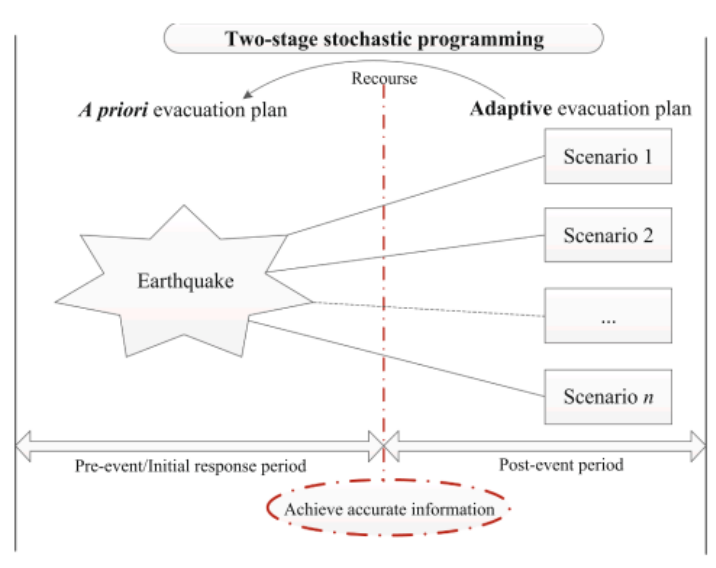
\includegraphics[scale =0.45]{2ss.png}
     \caption{Mô hình mô tả bài toán Stochastic for Evacuation}
     \label{fig:2ss}
 \end{figure}
 
 
Dựa vào hình trên thì ta có thể dễ dàng thấy và hiểu ra rằng bài toán này có 2 giai đoạn sẽ được diễn ra , giai đoạn đầu được gọi là trước thảm họa - ở giai đoạn này chúng ta sẽ phải đưa ra các dự đoán , giả định những điều sẽ xảy ra ở giai đoạn 2 và giai đoạn này gọi là sau thảm họa , sẽ xảy ra rất nhiều scenario và mỗi scenario đều có xác suất xảy ra khác nhau, tương ứng xảy ra những sự kiện khác nhau do đó ở giai đoạn 1 chúng ta phải đưa ra những biện pháp ứng phó với các tình huống , sự kiện xảy ra ở giai đoạn 2 và nó cũng chính là bài toán 2-Stage Stochastic Programming mà chúng ta sẽ phân tích ở problem 2 này . Từ bài toán đó ta có thể tìm được con đường phù hợp nhất để người dân có thể di chuyển từ nơi nguy hiểm sang với nhiểu số lượng nhiểu nhất và tốn ít thời gian nhất tương ứng với capacity và timecost mà em đã đề cập ở trên.
 \subsubsection{Vấn đề luồng tối thiểu với chi phí nhỏ nhất (Minimum-Cost Flow Problem)}
Vấn đề luồng tối thiểu với chi phí nhỏ nhất (Minimum-Cost Flow Problem - MCFP) là một vấn đề tối ưu và quyết định để tìm cách gửi luồng với chi phí rẻ nhất thông qua một mạng lưu thông. Một ứng dụng điển hình của vấn đề này liên quan đến việc tìm đường giao hàng tốt nhất từ một nhà máy đến một kho hàng, trong đó mạng đường có một số khả năng và chi phí tương ứng. Vấn đề luồng tối thiểu với chi phí nhỏ nhất là một trong những vấn đề cơ bản nhất trong tất cả các vấn đề về luồng và tuần hoàn vì hầu hết các vấn đề khác có thể được chuyển thành vấn đề luồng tối thiểu với chi phí nhỏ nhất và cũng có thể được giải quyết hiệu quả bằng thuật toán mạng đơn giản.\\
Ví dụ tổng quát của bài toán :\\
Maximum flow problem with minimum cost :\\
Dữ liệu đầu vào:\\ 
\begin{minipage}{0.8\textwidth}
    \setlength{\parindent}{20pt}
    Đồ thị có hướng \textcolor{blue}{$G = (V, E)$} với đỉnh nguồn \textcolor{blue}{$s$} và đỉnh đích \textcolor{blue}{$t$}.

Hàm dung lượng \textcolor{blue}{$c: E \rightarrow \mathbb{R}$}, trong đó \textcolor{blue}{$c(u, v) \geq 0$} cho mọi cung \textcolor{blue}{$(u, v) \in E$}.

Hàm chi phí \textcolor{blue}{$a: E \rightarrow \mathbb{R}$, trong đó $a(u, v) \geq 0$} cho mọi cung \textcolor{blue}{$(u, v) \in E$}.
\end{minipage}\\
Mục tiêu:
\[
\begin{cases}
       \textcolor{blue}{f(u,v) \leq c(u,v),} \text{với tất cả} \textcolor{blue}{(u,v) \in E}\\ 
       
       \textcolor{blue}{\sum_{v \in V}  f(v,u) = \sum_{v\in V}  f(u,v),} \text{với} \textcolor{blue}{u \ne s,t}\\
       
       \textcolor{blue}{ \sum_{(u,v)\in E} a(u,v)f(u,v)} \text{nên được giảm thiểu}\\
\end{cases}
\]
\\
Vấn đề luồng tối thiểu với chi phí có thể được giải quyết bằng lập trình tuyến tính, vì chúng ta tối ưu hóa một hàm tuyến tính và tất cả các ràng buộc đều là tuyến tính.\\

Dưới đây là một số thuật toán cơ bản được biết đến (chúng có nhiều biến thể):\begin{itemize}
 \item \textcolor{blue}{Cycle Canceling}: Đây là một phương pháp cơ bản dựa trên phương pháp nguyên tố. Thuật toán này lặp lại việc hủy bỏ chu trình trong mạng dư còn đến khi đạt được luồng tối ưu. 
 \item \textcolor{blue}{Cut Canceling}: Đây là một phương pháp cơ bản dựa trên phương pháp kép. Thuật toán này lặp lại việc hủy bỏ cắt trong mạng dư còn đến khi đạt được luồng tối ưu. 
 \item \textcolor{blue}{Minimum Mean Cycle Canceling}: Đây là một thuật toán đơn giản và hiệu quả dựa trên đa thức mạnh. Thuật toán này hủy bỏ chu trình trung bình nhỏ nhất trong mạng dư còn. 
 \item \textcolor{blue}{Successive Shortest Path} và \textcolor{blue}{Capacity Scaling}: Đây là những phương pháp kép, có thể được coi là sự tổng quát hóa của thuật toán Ford-Fulkerson. Chúng liên quan đến việc tìm đường đi ngắn nhất trong mạng dư còn và tỷ lệ khả năng để đạt được luồng tối ưu. 
 \item \textcolor{blue}{Cost Scaling}: Đây là một phương pháp nguyên tố kép, coi là sự tổng quát hóa của thuật toán đẩy-lấy. Phương pháp này liên quan đến việc tăng cường luồng theo các cung dư có chi phí rẻ nhất. 
 \item \textcolor{blue}{Network Simplex Algorithm}: Đây là một phiên bản đặc biệt của phương pháp simplex trong lập trình tuyến tính, được điều chỉnh để giải quyết các vấn đề luồng mạng. 
 \item \textcolor{blue}{Out-of-Kilter Algorithm}: Đây là một phương pháp nguyên tố khác, được phát triển bởi D.R. Fulkerson, điều chỉnh luồng theo các cung dư để cải thiện tính tối ưu cho đến khi đạt được luồng tối ưu. 
\end{itemize}

Các thuật toán này có những điểm mạnh yếu khác nhau về hiệu suất và độ phức tạp của việc triển khai, và sự lựa chọn thuật toán phụ thuộc vào các đặc điểm cụ thể của vấn đề và các tài nguyên có sẵn. 

Ở bài báo cáo này , chúng ta sẽ trình bày hai giải thuật là Successive Shortest Path và Cycle Canceling .Đồng thời so sánh độ hiệu quả của chúng .

Residual network là một yếu tố không thể thiếu của 2 giải thuật trên , giúp chúng ta tìm ra chu trình âm và loại bỏ nó bằng thuật toán Bellman-Ford . Để tạo ra nó thì cũng khá đơn giản , giả sử ta có đồ thị G và các luồng trên cạnh ij là \textcolor{blue}{$x_{i j}$} thỏa mãn điều kiện \textcolor{blue}{$x_{i j} \leqslant  u_{i j}$}( luồng tối đa có thể qua cạnh đó ) và tương ứng với từng cạnh ij ấy ta sẽ có \textcolor{blue}{$c_{i j}$} - flow cost( luồng chi phí) . Từ đó ta có được \textcolor{blue}{$r_{ij}$}( residual capacity) của từng cạnh theo công thức \textcolor{blue}{$r_{i j} = u_{i j} - x_{i j}$} , nếu chúng ta gửi nó theo đường i->j thì tức là sẽ thêm vào Node bất kì nào đó một lượng flow bằng \textcolor{blue}{$r_{i j}$} tương ứng khiến flowcost tăng lên \textcolor{blue}{$c_{i j}$} và ngược lại thì sẽ là giảm khiến flowcost giảm \textcolor{blue}{$c_{i j}$}.
   
\subsection{Mô tả model}
Từ mô hình ban đầu có thể thấy rằng ràng buộc ghép \textcolor{blue}{$\sum_{t \leqslant \widetilde{T}} y_{i j}^s(t)=x_{i j},(i, j) \in A, s=1,2, \cdots, S$}
là một ràng buộc cứng. Ràng buộc này đặc trưng cho mối quan hệ giữa việc lựa chọn một liên kết vật lý và các cung phụ thuộc thời gian dựa trên kịch bản tương ứng. Do đó, chúng tôi giới thiệu phương trình Lagrangian hệ số nhân \textcolor{blue}{$\alpha_{i j}^s(t),(i, j) \in A, s=1,2, \cdots, S, t \leqslant \widetilde{T}$} cho ràng buộc ghép nối, và sau đó ràng buộc này có thể được nới lỏng thành mục tiêu hàm dưới dạng sau: 
\textcolor{blue}{$\sum_{s=1}^S \sum_{t \leqslant \widetilde{T}} \sum_{(i, j) \in A} \alpha_{i j}^S(t)\left(y_{i j}^s(t)-x_{i j}\right)$}
Việc sử dụng nhân tử Lagrange vào bài toán có thể giúp tối ưu hóa một hàm mục tiêu với các ràng buộc liên quan đến quyết định về kế hoạch và việc sơ tán ngẫu nhiên. Do đó, sau khi nới lỏng công thức (12) thành hàm mục tiêu, công thức nới lỏng của mô hình (10) có thể được xây dựng như sau: 
\textcolor{blue}{$\left\{\begin{array}{l}\min \sum_{(i, j) \in A} p_{i j} x_{i j}+\sum_{s=1}^S\left(\mu_s \cdot \sum_{(i, j) \in A_s} c_{i j}^S(t) \cdot y_{i j}^s(t)\right)+ \\ \sum_{s=1}^S \sum_{t \leqslant \tilde{T}} \sum_{(i, j) \in A} \alpha_{i j}^S(t)\left(y_{i j}^s(t)-x_{i j}\right) \\ s . t . \\ \sum_{(i, j) \in A} x_{i j}-\sum_{(j, i) \in A} x_{i j}=d_i, \forall i \in V \\ 0 \leqslant x_{i j} \leqslant u_{i j}, \forall(i, j) \in A \\ \sum_{\left(i, j, j^{\prime}\right) \in A_s} y_{i j}^s(t)-\sum_{\left(j_{\left.t^{\prime}, i_t\right) \in A_s}\right.} y_{i j}^s\left(t^{\prime}\right)=d_i^s(t), \forall i \in V, \\ t \in\{0,1, \cdots, T\}, s=1,2, \cdots, S \\ 0 \leqslant y_{i j}^S(t) \leqslant u_{i j}^s(t), \forall(i, j) \in A, t \in\{0,1, \cdots, T\}, s=1,2, \cdots,\end{array}\right.$}

Nhìn vào mô hình 13 ta thấy các biến x và y có thể được được tách rời nhau, do đó ta có thể tách thành hai bài toán con sau: 

Bài toán con 1: Bài toán luồng chi phí tối thiểu  

Bài toán con đầu tiên có thể được coi là luồng chi phí tối thiểu bài toán và dạng của nó được cho như sau:

\textcolor{blue}{$\left\{\begin{array}{l}\min S P 1(\alpha)=\sum_{(i, j) \in A}\left(p_{i j}-\sum_{s=1}^S \sum_{t \leqslant \widetilde{T}} \alpha_{i j}^S(t)\right){x_{i j}} \\ \text { s.t. } \\ \sum_{(i, j) \in A} x_{i j}-\sum_{(j, i) \in A} x_{i j}=d_i, \forall i \in V \\ 0 \leqslant x_{i j} \leqslant u_{i j}, \forall(i, j) \in A\end{array}\right.$}

Hàm mục tiêu biểu thị một bài toán tối thiểu hóa chi phí, trong đó chi phí gắn liền với chệnh lệch giữa \textcolor{blue}{$p_{i j}$ và tổng ${\alpha}_{i j}^S(t)$} trên các chỉ số nhất định. Hàm mục tiêu có thể được định nghĩa từ \textcolor{blue}{$g_{i j}:=p_{i j}-\sum_{s=1}^S \sum_{t \leqslant \widetilde{T}} \alpha_{i j}^S(t)$} để biểu thị chi phí tổng quát của mỗi liên kết.

Với $p_{i j}$ là tham số ảnh hưởng đến quá trình tối ưu hóa bằng cách ấn định penalty hoặc cost cho mỗi liên kết trong mạng. The penalty function được thiết kế để giảm thiểu hoặc loại bỏ việc sử dụng các liên kết góp phần hình thành các vòng lặp hoặc các tuyến đi phụ trong quá trình sơ tán. 

\textcolor{blue}{$\sum_{s=1}^S \sum_{t \leqslant \widetilde{T}} \alpha_{i j}^S(t)\right$} biểu thức này là một tổng của biến Lagrange $a_{i j}$ qua tất cả các kịch bản s và thời điểm t trong mô hình. biến lagrange dùng để điều chỉnh $p_{i j}$ tương ứng với mức độ thỏa mãn của 2 ràng buộc bên dưới:  
\begin{itemize}
\item Ràng buộc bảo toàn dòng: 

    \begin{minipage}{0.8\textwidth}
    Mỗi nút I trong đồ thi phải thỏa mãn ràng buộc toàn dòng:
    
    \textcolor{blue}{$\sum_{(i, j) \in A} x_{i j}-\sum_{(j, i) \in A} x_{i j}=d_i, \forall i \in V \ $}

    Ràng buộc này đảm bảo rằng lượng dòng vào và ra khỏi mỗi nít đều phải cân bằng với nhu cầu tại $d_i$ nút đó. 
    \end{minipage}
\item Ràng buộc giới hạn dòng: 

    \begin{minipage}{0.8\textwidth}
    \textcolor{blue}{\ 0 \leqslant x_{i j} \leqslant u_{i j}, \forall(i, j) \in A\}
    
    Ràng buộc này đảm bảo rằng giá trị của mỗi lượng dòng tại các cạnh nằm trong khoảng từ 0 đến \textcolor{blue}{$u_ij$} đến giới hạn cho phép, giữ cho mô hình trong phạm vi thực tế và khả thi.
    \end{minipage}
\end{itemize}

Bài toán con 2: Bài toán luồng chi phí tối thiểu phụ thuộc vào thời gian 

Bài toán con thứ hai của mô hình trên liên quan đến các biến quyết định Y và giá trị mục tiêu tối ưu của bài toán được viết tắt là \textcolor{blue}{$Z^*_{SP2} (\alpha)$}, được thể hiện như sau: 

\textcolor{blue}{$\left\{\begin{array}{l}\min S P 2(\alpha)=\sum_{S=1}^S \sum_{(i, j) \in A}\left(\sum_{t \in\{0,1, \cdots, T\}} \mu_s \cdot c_{i j}^S(t)+\sum_{t \leqslant \widetilde{T}} \alpha_{i j}^S(t)\right) y_{i j}^S(t) \\ s . t . \\ \sum_{\left(i t, j_{t^{\prime}}\right) \in A_S} y_{i j}^S(t)-\sum_{\left(j_{t^{\prime}}, i_t\right) \in A_S} y_{i j}^S\left(t^{\prime}\right)=d_i^S(t), \forall i \in V, \\ t \in\{0,1, \cdots, T\}, s=1,2, \cdots, S \\ 0 \leqslant y_{i j}^S(t) \leqslant u_{i j}^S(t), \forall(i, j) \in A, t \in\{0,1, \cdots, T\}, s=1,2, \cdots, S\end{array}\right.$}

Mục tiêu là tối thiểu hóa tổng chi phí, bao gồm chi phí liên quan đến thời gian di chuyển và chi phí hạn chế tài nguyên, dựa trên xác suất của từng kịch bản và quyết định về lưu lượng trên mỗi liên kết. 



Algorithm 1: Thuật toán đường đi ngắn nhất liên tiếp cho bài toán luồng tối thiểu với chi phí nhỏ nhất:\\
\begin{minipage}{0.8\textwidth}
\setlength{\parindent}{20pt}
Bước 1: Chọn biến \textcolor{blue}{x} là một luồng khả thi giữa bất kỳ cặp điểm gốc-đích nào và có chi phí giao hàng nhỏ nhất trong các luồng khả thi có cùng giá trị luồng.

Bước 2: Thuật toán sẽ kết thúc nếu giá trị luồng \textcolor{blue}{x} đạt đến \textcolor{blue}{v} hoặc không có đường đi có chi phí nhỏ nhất trong mạng dư còn lại \textcolor{blue}{(V , A(x),C(x),U(x),D)};nếu không, đường đi ngắn nhất với luồng tối đa được tính bằng thuật toán đánh dấu đúng, sau đó chuyển đến  Bước 3. Các hàm \textcolor{blue}{A(x),C(x),U(x)} trong mạng dư có thể được định nghĩa như sau:
$$
\begin{aligned}
& \textcolor{blue}{A(x)=\left\{(i, j) \mid(i, j) \in A, x_{i j}<u_{i j}\right\} \cup\left\{(j, i) \mid(j, i) \in A, x_{i j} \geq 0\right\}} \\
& \textcolor{blue}{C(x) \equiv\left\{\begin{array}{l}
\bar{c}_{i j},(i, j) \in A, x_{i j}<u_{i j} \\
-c_{i j},(j, i) \in A, x_{j i}>0
\end{array}\right.} \\
&\textcolor{blue}{ U_{i j}(x)=}\left\{\begin{array}{l}
\textcolor{blue}{u_{i j},(i, j) \in A, x_{i j}<u_{i j}} \\
\textcolor{blue}{x_{j i},(j, i) \in A, x_{j i}>0}
\end{array}\right.
\end{aligned}
$$

Bước 3: Tăng giá trị luồng trên đường đi có chi phí nhỏ nhất. Nếu giá trị luồng tăng không vượt quá v, chuyển đến Bước 2.
\end{minipage}\\
\\
SubProblem 2 có thể được phân rã thành tổng cộng \textcolor{blue}{S} bài toán con, mỗi bài toán con có thể được gọi là bài toán luồng tối thiểu với thời gian di chuyển trên các liên kết và khả năng chứa của chúng phụ thuộc vào thời gian , cụ thể là : \\
$$
\left\{\begin{array}{l}
\textcolor{blue}{\min S P 2(\alpha, s)=\sum_{(i, j) \in A}\left(\sum_{t \in\{0,1, \cdots, T\}} \mu_s \cdot c_{i j}^s(t)+\sum_{t \leqslant \widetilde{T}} \alpha_{i j}^s(t)\right) y_{i j}^s(t)} \\
\textcolor{blue}{s . t . }\\
\textcolor{blue}{\sum_{\left(i_{t}, j_{t'}\right) \in A_s} y_{i j}^s(t)-\sum_{\left(j_{t'}, i_t\right) \in A_s} y_{i j}^s\left(t^{\prime}\right)=d_t^s(t), \forall i \in V, t \in\{0,1, \cdots, T\}} \\
\textcolor{blue}{0 \leqslant y_{i j}^s(t) \leqslant u_{i j}^s(t), \forall(i, j) \in A, t \in\{0,1, \cdots, T\}}
\hfill {(16)}
\end{array}\right.
$$

Với \textcolor{blue}{$d_{t}^s(t)$} biểu thị lưu lương tại thời điểm t và trong trường hợp s phụ thuộc vào thời gian.

\textcolor{blue}{$\alpha_{ij}^s(t)$}  larange trên liên kết i,j tại thời điểm t và trong trường hợp s phụ thuộc vào thời gian.\\

Đối với mỗi trường hợp \textcolor{blue}{$s\in\{{1,2,...S}\}$} bài toán con (16) có cách giải tương tự cấu trúc như bài toán con (14) với chi phí di chuyển trên liên kết \textcolor{blue}{$c_{ij}^s(t)$} và khả năng chứa liên kết \textcolor{blue}{${u_{ij}^s(t)}$} cũng như chi phí tổng quát \textcolor{blue}{$\mathbf{g}_{ij}^s(t)$} đều phụ thuộc vào thời gian . Vì khoảng thời gian T được chia thành hai giai đoạn thời gian, nên chi phí tổng quát được định nghĩa dưới dạng một hàm mảnh (piecewise  function) : \\
\textcolor{blue}{$$
g_{i j}^s(t)= \begin{cases}\mu_s \cdot c_{i j}^s(t)+\alpha_{i j}^s(t), & t \leqslant \widetilde{T} \\ \mu_s \cdot c_{i j}^s(t), & \widetilde{T}<t \leqslant T\end{cases}
$$}

Vì bài toán con (16) là bài toán luồng chi phí tối thiểu phụ thuộc vào thời gian, và do đó thuật toán 1 nên được sửa đổi ở Bước 2. Đầu tiên, các tham số \textcolor{blue}{A(y(t)), C(y(t)) và U(y(t))} trong mạng dư N(y)t)) được định nghĩa như sau:  
\[
\textcolor{blue}{\begin{aligned}
A_s(y(t)) &= \left\{(i_t, j_{t'}) \mid (i_t, j_{t'}) \in A_s, y_{ij}^s < u_{ij}^s \right\} \cup \left\{(j_{t'}, i_t) \mid (j_{t'}, i_t) \in A_s, y_{ij}^s > 0 \right\}, \\
s= 1,2, \cdots, S \\
c_{ij}^s(y(t)) &=
\begin{cases}
c_{ij}^s(t),  (i_t, j_{t'}) \in A_s, y_{ij}^s(t) < u_{ij}^s(t), t \in \{0,1,\cdots,T\} \\
-c_{ji}^s(t'), (j_{t'}, i_t) \in A_s, \forall\{t' \in \{0,1,\cdots,T\} \mid y_{ji}^s(t') > 0\},\\
 s = 1,2, \cdots, S,\\
 T, (j_{t'}, i_t) \in A_s, \forall\{t' \in \{0,1,\cdots,T\} \mid y_{ji}^s(t') = 0\}
\end{cases} \\
u_{ij}^s(y(t)) &=
\begin{cases}
u_{ij}^s(t) - y_{ij}^s(t),  (i_t, j_{t'}) \in A_s, y_{ij}^s(t) < u_{ij}^s(t), t \in \{1,2,\cdots,T\} \\
y_{ji}^s(t),  (j_{t'}, i_t) \in A_s, \forall\{t' \in \{0,1,\cdots,T\} \mid y_{ji}^s(t') > 0\}, \\
s = 1,2, \cdots, S \\
0,(j_{t'}, i_t) \in A_s, \forall\{t' \in \{0,1,\cdots,T\} \mid y_{ji}^s(t') = 0\}
\end{cases}
\end{aligned}}
\]
\\
Với:\\
\textcolor{blue}{N(y(t))} : mạng dư tại thời điểm \textcolor{blue}{t} với luồng hiện tại \textcolor{blue}{y(t)} \\
\textcolor{blue}{$c_{ij}^s(y(t))$} :thời gian di chuyển của liên kết \textcolor{blue}{(i, j)}  trong trường hợp s tại thời điểm t với luồng hiện tại \textcolor{blue}{y(t)} \\
\textcolor{blue}{$u_{ij}^s(y(t))$} :dung lượng của liên kết \textcolor{blue}{(i, j)} trong trường hợp s tại thời điểm t với luồng hiện tại \textcolor{blue}{y(t)} \\
$\textcolor{blue}{A_{s}(y(t)}$ : tập hợp các liên kết trong trường hợp tại thời điểm \textcolor{blue}{t} với luồng hiện tại \textcolor{blue}{y(t)} \\

Tiếp theo , Giải thuật label-correcting được sửa đổi sẽ được áp dụng để tìm đường đi có chi phí tối thiểu phụ thuộc vào thời gian trong mạng dư. Giải thuật label-correcting với mô tả cơ bản : 
\setlength{\parindent}{20pt}
\begin{enumerate}
  \item Khởi tạo mạng dư: Bắt đầu với mạng gốc, tạo mạng dư bằng cách gán giá trị vô cùng cho tất cả các cung và đặt chi phí ban đầu của các đỉnh khác vô cùng. 
  \item Khởi tạo đường đi: Đặt đỉnh xuất phát là đỉnh nguồn và gán chi phí ban đầu là 0. Các đỉnh khác được gán giá trị vô cùng.
  \item Lặp lại cho đến khi tìm được đường đi ngắn nhất đến đỉnh đích hoặc không còn đường đi hợp lệ:
    \begin{enumerate}[label=\textbf{\alph*.}]
  \item Tìm đỉnh chưa được xét có chi phí nhỏ nhất. Đây là đỉnh có giá trị nhỏ nhất trong tập các đỉnh chưa xét. 
  \item Cập nhật chi phí của các đỉnh kề với đỉnh hiện tại. Nếu chi phí đến đỉnh kề thông qua đỉnh hiện tại nhỏ hơn chi phí hiện tại, cập nhật chi phí mới và ghi nhận đỉnh hiện tại là đỉnh trước đó của đỉnh kề đó.
  \item Đánh dấu đỉnh hiện tại là đã xét.
    \end{enumerate}
   \item Kiểm tra kết quả:
   \begin{enumerate}[label=\textbf{\alph*.}]
  \item Nếu đỉnh đích không được đánh dấu là đã xét, không có đường đi từ đỉnh xuất phát đến đỉnh đích trong mạng. 
  \item Nếu đỉnh đích được đánh dấu là đã xét, truy vết đường đi từ đỉnh đích ngược về đỉnh xuất phát bằng cách sử dụng các đỉnh trước đó đã ghi nhận.
    \end{enumerate}
   \item Kết thúc: Trả về đường đi có chi phí tối thiểu từ đỉnh xuất phát đến đỉnh đích trong mạng. 
\end{enumerate}

Giải thuật này sẽ tìm kiếm và cập nhật chi phí của các đỉnh trong mạng dựa trên chi phí hiện tại và chi phí của các cung kề. Quá trình này sẽ lặp lại cho đến khi đạt được đỉnh đích hoặc không còn đường đi hợp lệ. 


Bằng cách giải các bài toán phụ (14) và (15) với giải pháp thư giãn X và Y, giá trị mục tiêu tối ưu ZLR cho mô hình thư giãn (13) với một vectơ đa chỉ Lagrange đã cho có thể được biểu diễn như sau:\\
\textcolor{blue}{$$Z_{LR}^*(\alpha) = Z_{SP1}^*(\alpha) + Z_{SP2}^*(\alpha)$$}\\
Rõ ràng, giá trị mục tiêu tối ưu của mô hình thư giãn (13) là giới hạn dưới của giá trị mục tiêu tối ưu của mô hình gốc (10). Để đạt được một giải pháp chất lượng cao, cần thiết phải đạt được một giới hạn dưới gần với giá trị mục tiêu tối ưu của mô hình gốc. Điều đó có nghĩa là cần đạt được giới hạn dưới lớn nhất có thể, và biểu thức được cho như sau: \\
\textcolor{blue}{$$Z_{LD}(\alpha ^ *) = max_{\alpha \geq 0} Z_{LR}(\alpha)$$}  \\
 Biểu thức trên có ý nghĩa là chúng ta tìm giá trị \textcolor{blue}{$\alpha^*$} không âm lớn nhất \textcolor{blue}{($max_{\alpha \geq 0}$)} sao cho giá trị mục tiêu tối ưu \textcolor{blue}{$Z_{LR}(\alpha)$} đạt được giới hạn dưới lớn nhất. \\
 Trong đó :\\
 \begin{itemize}
     \item \textcolor{blue}{$Z_{LD}(\alpha ^ *)$} là giá trị mục tiêu tối ưu của mô hình gốc (10) với giới hạn dưới lớn nhất (greatest lower bound). \\
     \item \textcolor{blue}{$Z_{LR}(\alpha^*)$} là giá trị mục tiêu tối ưu của mô hình thư giãn (13) với một giá trị alpha cụ thể. Đây là một giá trị được tính toán trong quá trình giải quyết mô hình thư giãn.\\
     \item Vì giá trị \textcolor{blue}{$\alpha^*$} được chọn là giá trị không âm lớn nhất, nên \textcolor{blue}{$Z_{LR}(\alpha^*)$} sẽ là giới hạn dưới tốt nhất có thể đạt được, sát với giá trị mục tiêu tối ưu của mô hình gốc. Điều này giúp xác định một giá trị ước lượng tốt cho giá trị mục tiêu tối ưu của mô hình gốc và hướng dẫn quá trình tìm kiếm giải pháp chất lượng cao.\\
 \end{itemize}

 \subsection{Trình bày giải thuật}
 Mô hình bài toán con 1 được mô tả phía trên còn được gọi là Successive Shortest Path Algorithm. Sau đây em sẽ trình bày 1 ví dụ được giải quyết bới thuật toán trên:

 \begin{center}
  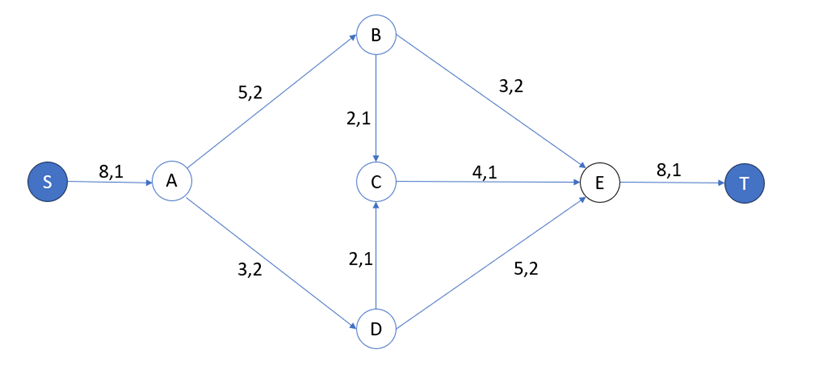
\includegraphics[height=7cm]{Picture1.png}
\end{center}
 Đầu tiên, ta dùng thuật toán Bellman – Ford để tìm luồng đi từ \textcolor{blue}{S} đến \textcolor{blue}{T} có chi phí nhỏ nhất và ta tìm được luồng \textcolor{blue}{S -> A -> B -> C -> E -> T} có chi phí nhỏ nhất là bằng 6 . Tiếp theo ta tìm capacity lớn nhất có thể truyền qua luồng này và có thể thấy là 2. Từ đó ta tính được cost của luồng này là 2*1+2*2+2*1+2*1+2*1 = 12. Và ta cũng có Residual Network:
\begin{center}
  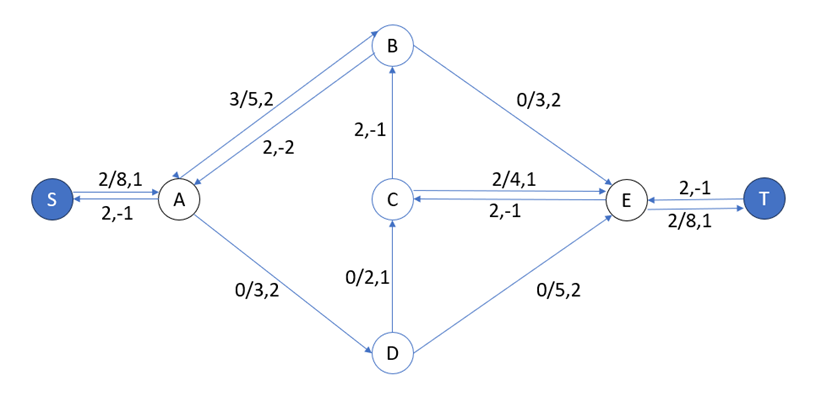
\includegraphics[height=7cm]{Picture2.png}
\end{center}
 Ta sử dụng Bellman – Ford để kiểm tra xem có chu trình âm hay không. Và mô hình trên không xuất hiện chu trình âm. Tiếp theo, ta dùng thuật toán Bellman – Ford để tìm luồng có chi phí nhỏ nhất. Tương tự như cách làm trên, ta tìm được luồng \textcolor{blue}{S -> A -> B -> E -> T} có chí phí nhỏ nhất là 4 và capacity lớn nhất có thể truyền qua là 3. Từ đó ta tính được cost hiện tại sẽ là \textcolor{blue}{12 + (3*1+3*2+3*2+3*1) = 30}. Sau đó, ta cập nhật lại Residual Network:
\begin{center}
  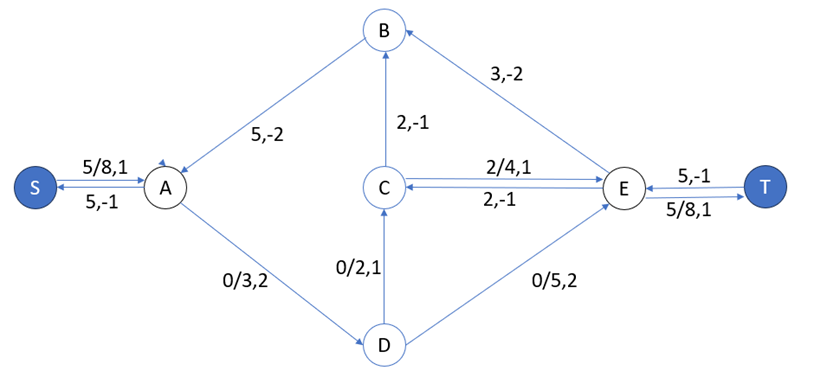
\includegraphics[height=7cm]{Picture3.png}
\end{center}
 Ta tiếp tục dùng Bellman – Ford để kiểm tra có chu trình âm hay không, ở đây ta không thấy xuất hiện chu trình âm nào cả. Lặp lại tương tự các bước như trên, ta sẽ tìm được luồng thỏa mãn tiếp theo là \textcolor{blue}{S -> A -> D -> C -> E -> T} có chi phí nhỏ nhất là 6 và capacity lớn nhất có thể truyền qua là 2. Ta cập nhật lại giá trị của cost sẽ là \textcolor{blue}{30 + (2*1+2*2+2*1+2*1+2*1) = 42}. Lúc này Residual Network cũng được cập nhật:
\begin{center}
  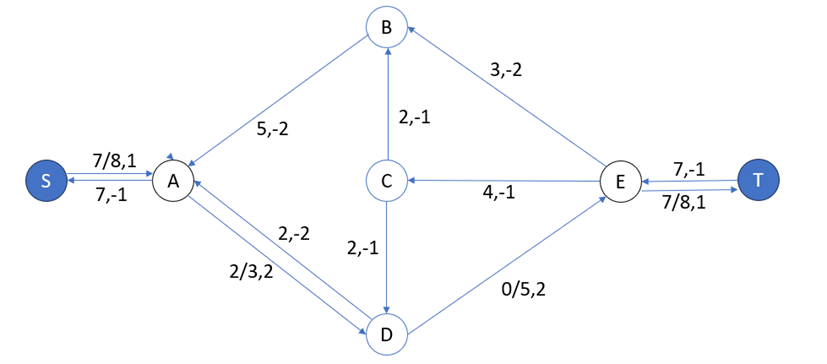
\includegraphics[height=7cm]{Picture4.png}
\end{center}
 Ta tiếp tục kiểm tra chu trình âm và thấy không xuất hiện chu trình âm. Tiếp tục làm tương tự như các bước trên, ta tìm được luồng là \textcolor{blue}{S -> A -> D -> E -> T}  và cập nhật giá trị của cost là \textcolor{blue}{42 + (1*1+1*2+1*2+1*1) = 48}. Ta cũng cập nhật lại Residual Network:
\begin{center}
  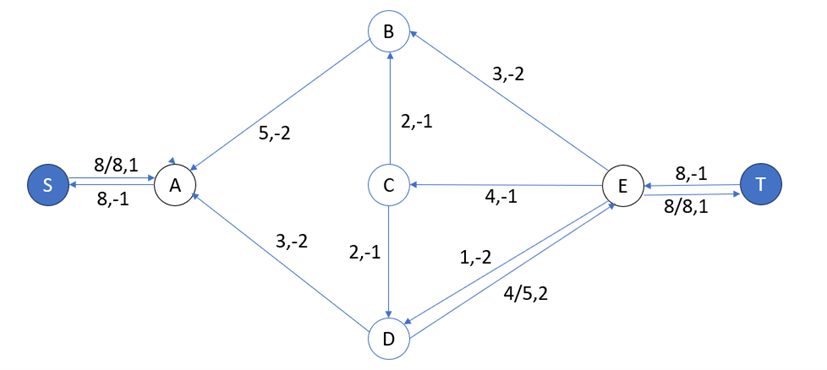
\includegraphics[height=7cm]{Picture5.png}
\end{center}
 Tương tự như trên, ta tiếp tục kiểm tra thấy không có chu trình âm và không còn đường đi từ S đến T nữa. Vậy ta có thể kết luận min cost của bài toán trên là 48.\\
 
 Ví dụ giải thuật Cycle Canceling : \\
 Ban đầu , ta tự tìm hoặc tạo một feasible flow trong đồ thị . Và ở phía dưới thì ta có thể dễ dàng thấy đó cũng chính là maxflow . Với tổng flow = 36 và cost = 48.
 \begin{center}
  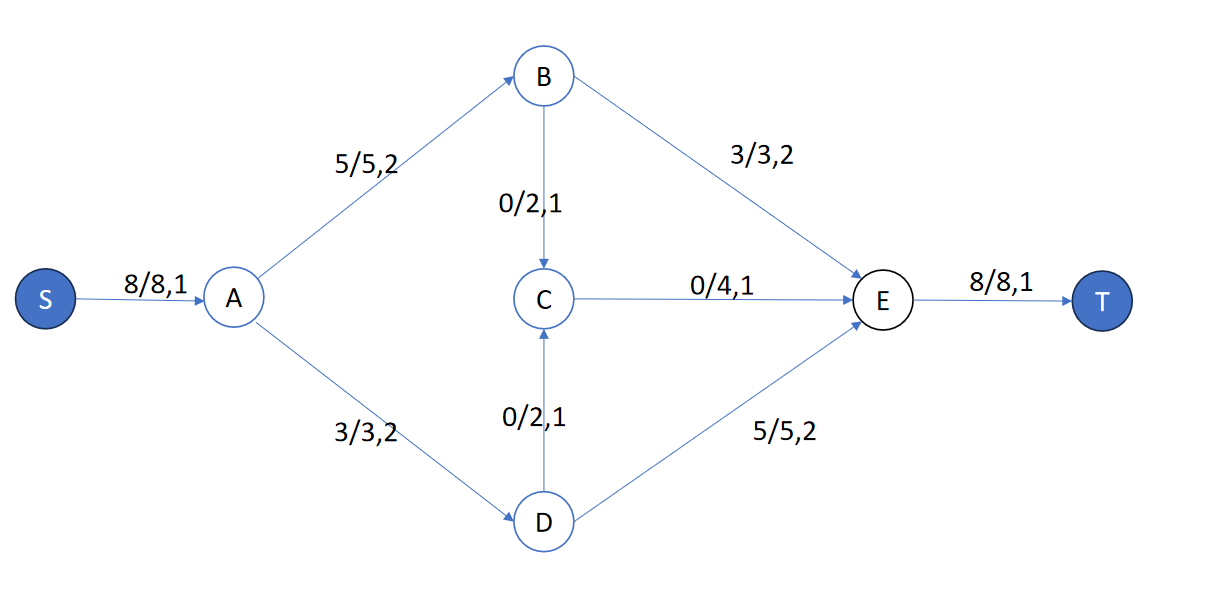
\includegraphics[height=7cm]{picture11.png}
\end{center}
Sau đó , ta tiến hành tìm chu trình âm trên đồ thị trên và loại bỏ nó . Hình phía dưới là quá trình biến đổi và tìm chu trình âm bằng giải thuật Bellman-Ford .
\begin{center}
  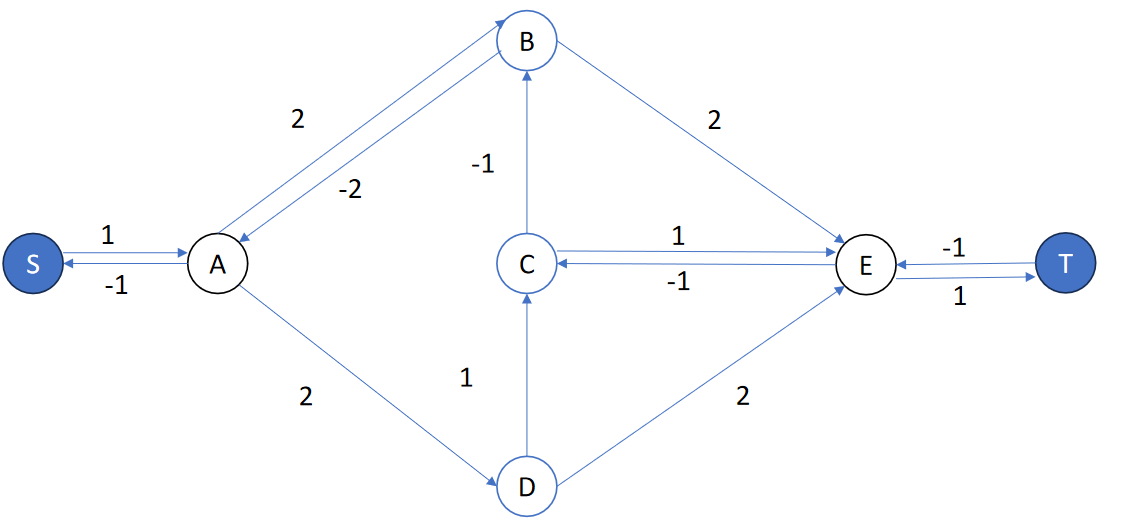
\includegraphics[height=7cm]{picture22.png}
\end{center}
Tương tự như vậy , thì không tìm thấy bất kì chu trình âm nào trong đồ thị trên.Vậy nên ta được Maxflow = 36 và mincost = 48 . Và để có ví dụ về  chu trình âm thì em giảm cost của BE xuống 1 và ta có thể thấy xuất hiện chu trình âm đó là B,E,C với 1 - 1 - 1 = -1 . Trường hợp xuất hiện chu trình âm thì ta tiến hành tăng lưu lượng trên các flow theo chiều thuận và giảm theo chiều nghịch bằng với giá trị vừa tăng - ở trường hợp giả định này thì ta sẽ tăng lưu lượng \textcolor{blue}{BE} và giảm trên \textcolor{blue}{EC} và \textcolor{blue}{BC}. Sau đó thì tiến hành lại bước đầu tiên đó là tìm ra feasible flow rồi tìm chu trình âm và loại bỏ cho đến khi không xuất hiện nữa .\\

Tóm lại thì giải thuật Cycle Canceling sẽ được thực hiện như sau :\\

\begin{minipage}{0.8\textwidth}
\setlength{\parindent}{20pt}
Bước 1: Tìm ra một feasible flow bất kì (tốt nhất nên tìm một cái maxflow vì bài toán chúng ta đang cần giải là maxflow mincost ) 

Bước 2 : Dùng thuật toán để tìm ra chu trình âm và loại bỏ nó bằng cách tăng lưu lượng trên các flow theo chiều thuận và ngược lại thì giảm , rồi tiếp tục quay lại bước 1. Điều kiện dừng của thuật toán này khi và chỉ khi đồ thị không có chứa bất kì chu trình âm nào.
\end{minipage}\\  

 
 \subsection{Mô tả giải thuật}
 Mô tả cơ bản giải thuật Successive shortest path :\\
 File source code chi tiết \textcolor{blue}{successive\_shortest\_path.py} đã được đính kèm cùng bài báo cáo này. 
\begin{lstlisting}[language=Python, caption={}, label={lst:pythoncode}]
function BellmanFord(start, n, flow, capacity, cost):
    distance = [infinity] * n
    distance[start] = 0
    parent = [-1] * n

    repeat n times:
        repeat for each u in range(n):
            repeat for each v in range(n):
                if flow[u][v] < capacity[u][v]:
                    if distance[u] + cost[u][v] < distance[v]:
                        distance[v] = distance[u] + cost[u][v]
                        parent[v] = u

    return distance, parent

function SuccessiveShortestPath(capacity, start, destination, cost):
    n = length(capacity)
    flow = createMatrix(n, n, 0)

    repeat forever:
        distance, parent = BellmanFord(start, n, flow, capacity, cost)
        if distance[destination] == infinity:
            break

        delta = infinity
        v = destination
        
        repeat while v is not start:
            u = parent[v]
            delta = min(delta, capacity[u][v] - flow[u][v])
            v = u

        v = destination

        repeat while v is not start:
            u = parent[v]
            flow[u][v] += delta
            flow[v][u] -= delta
            v = u

    total_cost = 0
    repeat for each u in range(n):
        repeat for each v in range(n):
            total_cost += flow[u][v] * cost[u][v]

    return total_cost, flow

\end{lstlisting}
 Mô tả cơ bản giải thuật Cycle Canceling :\\
 File source code chi tiết \textcolor{blue}{cyclecancling.py} đã được đính kèm với bài báo cáo này
\begin{lstlisting}[language=Python, caption={}, label={lst:pythoncode}]
    #Create or find any feasible flow, and make it the initial_flow
    #function cycle_cancelling(graph, cost, initial_flow): 
    n = graph.number_of_nodes() 
    flow = create_array(initial_flow) 
    #function find_negative_cycle(): 
        dist = create_array(float('inf'), n) 
        parent = create_array(-1, n) 
        source = 0 
        dist[source] = 0 
        for _ in range(n): 
            for each edge (u, v) in graph.edges(): 
                if graph[u][v]['capacity'] > 0 and dist[u] + cost[u][v] < dist[v]: 
                    dist[v] = dist[u] + cost[u][v] 
                    parent[v] = u 
                    
        for each edge (u, v) in graph.edges(): 
            if graph[u][v]['capacity'] > 0 and dist[u] + cost[u][v] < dist[v]: 
                cycle = [v] 
                while cycle[0] != v or length(cycle) <= 1: 
                    insert parent[cycle[0]] at the beginning of cycle 
                return cycle 
                
        return None 
        
    while True: 
        negative_cycle = find_negative_cycle() 
        if negative_cycle is None: 
            break 
        delta = minimum value of graph[u][v]['capacity'] for each edge (u, v) in negative_cycle 
        for each edge (u, v) in negative_cycle: 
            flow[u][v] += delta 
            flow[v][u] -= delta 
            graph[u][v]['capacity'] -= delta 
            graph[v][u]['capacity'] += delta 

    return flow 

final_flow = cycle_cancelling(graph, cost, initial_flow)  
min_cost = 0 
for (u, v) in graph.edges(): 
    min_cost += final_flow[u][v] * cost[u][v]  
\end{lstlisting}
    

Ví dụ :\\
Input :\begin{verbatim}
capacity = [                               cost = [
    [0, 4, 2, 0],                           [0, 2, 2, 0],
    [0, 0, 2, 3],                           [0, 0, 1, 3],
    [0, 0, 0, 5],                           [0, 0, 0, 1], 
    [0, 0, 0, 0]                            [0, 0, 0, 0] 
]                                       ]

Output :  
Final flow:[
    [0, 4, 2, 0,]
    [0, 0, 2, 2,]          
    [0, 0, 0, 4,]
    [0, 0, 0, 0,]
 ]
 Min cost: 24.0
\end{verbatim}
\subsection{So sách các giải thuật đã tìm hiểu}
\subsubsection{Tổng quan}
\begin{enumerate}
    \item \textbf{Successive Shortest Path:}
    \begin{itemize}
        \item \textbf{Thời gian:} Thuật toán ở đây chủ yếu có độ phức tạp mũ theo kích thước của đầu vào. Cụ thể, trong trường hợp xấu nhất, nó chỉ có thể đẩy tối đa $1$ đơn vị dòng trong mỗi vòng lặp, mất \textcolor{blue}{$O(F)$} vòng lặp để tìm một dòng có chi phí tối thiểu có kích thước \textcolor{blue}{$F$}, tổng thời gian chạy là \textcolor{blue}{$O(F \cdot T)$}, trong đó \textcolor{blue}{$T$} là thời gian cần để tìm đường đi ngắn nhất từ nguồn đến đích.

        Nếu thuật toán \textcolor{blue}{Bellman-Ford} được sử dụng, thời gian chạy trở thành \textcolor{blue}{$O(Fmn)$}. Cũng có thể sửa đổi thuật toán Dijkstra sao cho nó cần \textcolor{blue}{$O(nm)$} tiền xử lý làm bước ban đầu và sau đó hoạt động trong \textcolor{blue}{$O(m \log n)$} mỗi vòng lặp, tổng thời gian chạy là \textcolor{blue}{$O(mn + F m \log n)$}. Dưới đây là một đồ thị mẫu, trên đó thuật toán như vậy sẽ yêu cầu \textcolor{blue}{$O(2^{n/2} n^2 \log n)$} thời gian.
        

        \item \textbf{Không gian:} \textcolor{blue}{$O(V^2)$} để lưu trữ đồ thị và các cấu trúc dữ liệu khác.
    \end{itemize}
    \item \textbf{Cycle canceling}
    \begin{itemize}
        \item \textbf{Thời gian:} Đặt \textcolor{blue}{\(C\)} là sức chứa tối đa của các cạnh trong mạng, \textcolor{blue}{\(P\)} là chi phí tối đa của các cạnh trong mạng, và \textcolor{blue}{\(E\)} là số lượng cạnh. Sau đó, tổng chi phí của luồng ở đầu của thuật toán không vượt quá \textcolor{blue}{\(C \cdot P \cdot E\)}. Trong trường hợp xấu nhất, ở mỗi vòng lặp, bạn giảm tổng chi phí đi 1 đơn vị sau khi tìm thấy chu kỳ âm. Vì chi phí không thể là số âm, điều này dẫn chúng ta tối đa \textcolor{blue}{\(C \cdot P \cdot E\)} vòng lặp. Đối với việc tìm chu kỳ âm, bạn có thể sử dụng thuật toán Bellman-Ford, độ phức tạp của nó là \textcolor{blue}{\(O(VE)\)}, trong đó \textcolor{blue}{\(V\)} là số đỉnh trong một mạng. Do đó, độ phức tạp tổng của thuật toán hủy chu kỳ là \textcolor{blue}{\(O(E^2VCP)\)}.
        \item \textbf{Không gian:} \textcolor{blue}{$O(E+V)$} để lưu trữ các biến và cấu trúc dữ liệu phụ.

    \end{itemize}
\end{enumerate}
\subsubsection{Thực nghiệm}
    \begin{enumerate}
        \item \textbf{Source code}\\
        File source code chi tiết \textcolor{blue}{comparison.py, main.ipynb} đã được đính kèm cùng bài báo cáo này.
        %\hyperlink{https://github.com/NguyenBk22/Mathematical-Modeling-Assignment-2023}%{https://github.com/NguyenBk22/Mathematical-Modeling-Assignment-2023}
        \item \textbf{Tạo đồ thị}
        Trong bài tập lớn này, nhóm sử dụng thư viện networkx để tạo đồ thị có hướng. Nhóm thực hiện tạo capacity và cost dựa trên random với capacity có miền giá (1,10) và cost có miền giá trị (1,5).
        \begin{figure} [H]
            \centering
            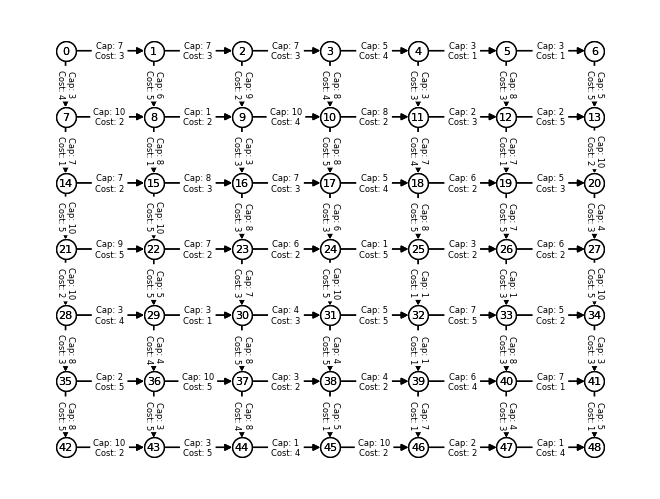
\includegraphics[width=\textwidth]{output.png}
            \caption{Hình ảnh đồ thị trước khi chạy giải thuật}
            \label{fig:h2}
        \end{figure} \\
        Ở hình \ref{fig:h2} là đồ thị dạng lưới với (row, col) là (7,7) tổng cộng là 49 node.\\
        \begin{figure} [H]
            \centering
            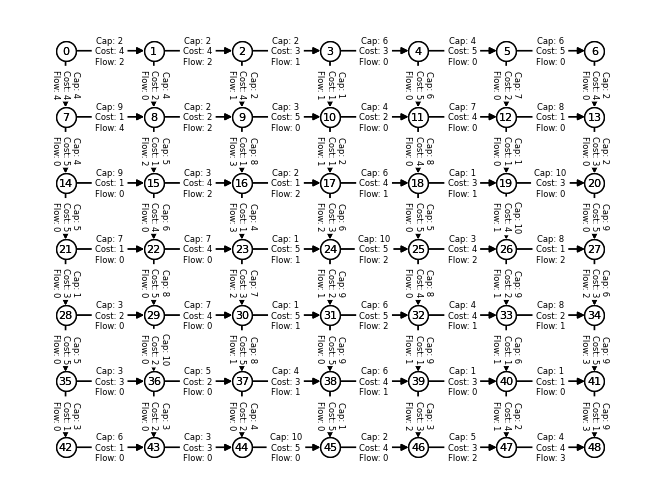
\includegraphics[width=1\linewidth]{image3.png}
            \caption{Kết quả sau khi thực hiện giải thuật}
            \label{fig:h3}
        \end{figure}
        
        Hình bên trên là kết quả sau khi chạy giải thuật để tìm min cost flow.
        
        \item \textbf{So sánh}
        
        Nhóm đã hiện thực hàm \textcolor{blue}{compare\_2\_algorithms} để so sánh 2 giải thuật và hàm reshape để tạo lại grid NxN. Dưới đây là phần code để so sánh 2 giải thuật.
        \begin{figure}[H]
            \centering
            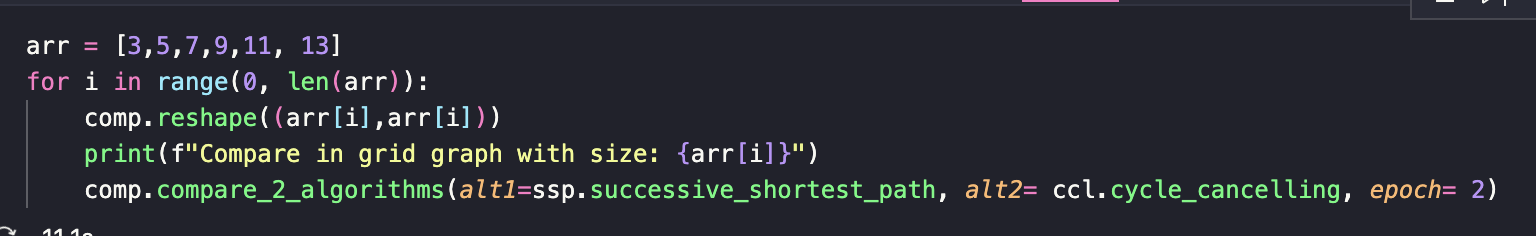
\includegraphics[width=\linewidth]{image.png}
        \end{figure}

        \newpage
        Hàm \textcolor{blue}{compare\_2\_algorithms} nhận vào lần lượt giải thuật 1 và 2,  \textcolor{blue}{epoch} là số lần chạy so sánh. Kết quả thực hiện được thể hiện ở hình bên dưới.
        \begin{figure}[H]
            \centering
            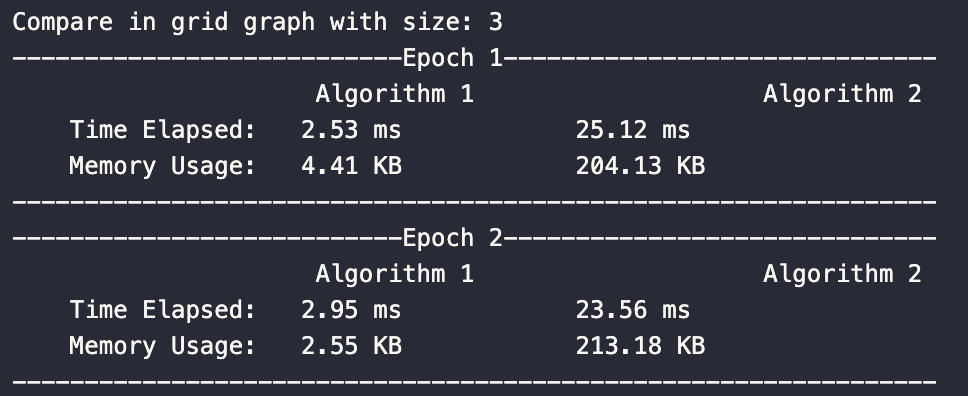
\includegraphics[width=1\linewidth]{compare.png}
            \caption{Kết quả với grid 3x3}
            \label{fig:h3}
        \end{figure}

        \textbf{Bảng so sánh:}
        \begin{table}[H]
            \centering
            \caption{So sánh giải thuật trên đồ thị grid}
            \begin{tabular}{|c|c|c|c|c|}
                \hline
                \multirow{2}{*}{Grid Size} & \multicolumn{2}{c|}{Successive shortest path} & \multicolumn{2}{c|}{Cycle cancelling} \\
                \cline{2-5}
                & Time Elapsed (ms) & Memory Usage (KB) & Time Elapsed (ms) & Memory Usage (KB) \\
                \hline
                3 & 2.53 & 4.41 & 25.12 & 204.13 \\
                \hline
                5 & 70.42 & 474.49 & 748.93 & 2172.00 \\
                \hline
                7 & 367.86 & 1577.66 & 4884.05 & 12928.54 \\
                \hline
                9 & 1946.67 & 5349.41 & 23281.15 & 50632.07 \\
                \hline
                11 & 14601.17 & 17112.62 & 82741.45 & 160403.73 \\
                \hline
                13 & 47119.30 & 54479.99 & 236649.47 & 398141.20 \\
                \hline
            \end{tabular}
            \label{tab:comparison}
        \end{table}
        
         Qua bảng so sánh ta thấy được về thời gian và dung lượng bộ nhớ sử dụng thì giải thuật Successive shortest path mà nhóm đã hiện thực luôn tốt, hiểu quả hơn so với giải thuật Cycle canceling trên đồ thị dạng lưới. 
    \end{enumerate} 
    

\newpage
\section{Reference}
\text[1] Refrence \textit{Simple linear programming model}, truy cập từ:  \url{https://gamspy.readthedocs.io/en/latest/examples/model_lib/SimpleLP.html#simplelp}\\
\text{[2] A. Shapiro, D. Dentcheva, and A. Ruszczynski, \textit{Lectures on stochastic programming: modeling}}\\
\text{\textit{and theory}. SIAM, 2021.}\\
\text[3]  L. Wang, “A two-stage stochastic programming framework for evacuation planning in disaster responses”, \textit{Computers \& Industrial Engineering}, vol. 145, p. 106458, 2020.\\
\text[4] Zealint, \textit{MINIMUM COST FLOW PART TWO: ALGORITHMS}, try cập từ:
\url{https://www.topcoder.com/thrive/articles/Minimum%20Cost%20Flow%20Part%20Tw%20Algorithms?fbclid=IwAR3RXCydz_2wGlBTvtaprBC1nxE94qac1V4iFXc1sP-QPuLik2Ng5nCdes0#1}
\end{document}

